\documentclass{beamer}
\usepackage{graphicx}
\usepackage{listings}

\lstdefinestyle{basic}{showstringspaces=false,
                       columns=fullflexible,
                       language=C++,
                       escapechar=@,
                       basicstyle=\tiny\sffamily,
classoffset=1,
morekeywords={pfunc_cilk_task_init, pfunc_cilk_task_clear},
morekeywords={pfunc_cilk_spawn_c, pfunc_cilk_wait, pfunc_cilk_task_t},
keywordstyle=[1]\color{blue}, 
classoffset=0,
moredelim=**[is][\color{white}]{~}{~},
literate={->}{{$\rightarrow\;$}}1 {<-}{{$\leftarrow\;$}}1 {=>}{{$\Rightarrow\;$}}1,
}
\lstset{language=C++,style=basic}

\newenvironment{discuss}{\begin{list}{}{}\item[]{\it Discussion item:}
\addcontentsline{toc}{subsection}{Discussion Item}
}{{\rm ({\it End of discussion item.})} \end{list}}
\newcommand{\code}[1]{\lstinline[basicstyle=\sffamily]{#1}}
\newcommand{\func}[1]{\lstinline[basicstyle=\sffamily]{#1()}}
\newcommand{\Cpp}{C\kern-0.05em\texttt{+\kern-0.03em+}}
\newcommand{\MPIpp}{MPI\kern-0.05em\texttt{+\kern-0.03em+}}
\newcommand{\tablefont}{\fontsize{8}{13}\selectfont}
\newcommand{\halfline}{\vspace{-1.0ex}}

\mode<presentation>
{
  \usetheme{Warsaw}
  \setbeamercovered{transparent}
  \definecolor{TUCGreen}{RGB}{0,100,50}
  \definecolor{TUCGreenlight}{RGB}{120,200,150}
  \definecolor{IURed}{RGB}{255,0,0}
  \definecolor{IURedlight}{RGB}{255,204,204}
  \definecolor{OMPIBlue}{RGB}{80,130,255}
  \definecolor{OMPIBluelight}{RGB}{240,240,255}
  \definecolor{white}{RGB}{255,255,255}
  \definecolor{black}{RGB}{0,0,0}
  \setbeamercolor*{palette primary}{fg=white, bg=IURed}
  \setbeamercolor*{palette secondary}{fg=white, bg=IURed}
  \setbeamercolor*{palette tertiary}{fg=white, bg=IURed}
  \setbeamercolor*{palette quartenary}{fg=white, bg=IURed}
  \setbeamercolor*{palette sidebar primary}{fg=white, bg=IURed}
  \setbeamercolor*{palette sidebar secondary}{fg=white, bg=IURed}
  \setbeamercolor*{palette sidebar tertiary}{fg=white, bg=IURed}
  \setbeamercolor*{palette sidebar quartenary}{fg=white, bg=IURed}
  \setbeamercolor*{normal text}{fg=black, bg=white}
  \setbeamercolor*{example text}{fg=black, bg=white}
  \setbeamercolor*{titlelike}{fg=white, bg=IURed}
  \setbeamercolor*{separation line}{fg=white, bg=IURed}
  \setbeamercolor*{item projected}{fg=white, bg=IURed}
  \setbeamercolor*{block title}{fg=white, bg=IURed}
  \setbeamercolor*{block title alerted}{fg=IURed, bg=white}
  \setbeamercolor*{block title example}{fg=IURed, bg=white}
  \setbeamercolor{block body}{fg=black, bg=IURedlight}
  \setbeamercolor*{structure}{fg=IURed, bg=white}
  \setbeamercolor*{sidebar}{fg=IURed, bg=white}
}

\usepackage[english]{babel}
\usepackage[latin1]{inputenc}
\usepackage{times}
\usepackage[T1]{fontenc}

\title{PFunc: Modern Task Parallelism For Modern HPC}

\author{Prabhanjan ``Anju'' Kambadur}

\date{{\small IBM T J Watson Research Center}\\
{\footnotesize Yorktown Heights, NY}\\
$20^{th}$ July 2009}

\begin{document}

\begin{frame}
  \titlepage
\end{frame}

\begin{frame}
\frametitle{Motivation}
\begin{itemize}
\item Parallelize a wide-variety of applications.
  \begin{itemize}
  \item Traditional HPC, informatics and mainstream.
  \end{itemize}
\item Parallelize for modern architectures.
  \begin{itemize}
  \item Multi-core, many-core and GPGPUs.
  \end{itemize}
\item Enable user-driven optimizations.
  \begin{itemize}
  \item Fine-tune application performance.
  \item No runtime penalties.
  \end{itemize}
\item Mix SPMD-style programming with tasks.
  \begin{itemize}
  \item Traditionally reserved only for distributed-memory.
  \end{itemize}
\end{itemize}
\end{frame}

\begin{frame}
\frametitle{What is PFunc}
\begin{itemize}
\item Task parallel library.
  \begin{itemize}
  \item C and \textcolor{blue}{\Cpp{}} APIs.
  \end{itemize}
\item Extends existing task parallel feature-set. 
  \begin{itemize}
  \item Cilk, Threading Building Blocks (TBB), Fortran M, etc.
  \end{itemize}
\item Portable.
  \begin{itemize}
  \item Linux, OS X, AIX and Windows.
  \end{itemize}
\item Highly customizable.
  \begin{itemize}
  \item Generic and generative programming techniques.
  \item \textcolor{blue}{No runtime penalty for customization!}
    \begin{itemize}
    \item \Cpp{} Standard Library (SL) and Boost Libraries.
    \end{itemize}
  \end{itemize}
\end{itemize}
\end{frame}

\begin{frame}[fragile]
\frametitle{Roadmap}
\begin{itemize}
\item $10,000$ foot view of PFunc.
\item Generating a PFunc library instance description.
\item Features of PFunc: 
  \begin{itemize}
  \item \textcolor{blue}{taskmgr, task, attribute, group.}
  \end{itemize}
\item Fibonacci example.
\item If time permits:
  \begin{itemize}
  \item Exception handling.
  \item Performance monitoring with PAPI.
  \item Performance results.
    \begin{itemize}
    \item \textcolor{red}{Really pushing it!}
    \end{itemize}
  \end{itemize}
\end{itemize}
\begin{center}
$\rightarrow{}$ \textcolor{green}{Help you parallelize applications with PFunc!}
\end{center}
\end{frame}

\begin{frame}
\frametitle{Overview}
\begin{figure}[t]
\centering
\includegraphics[width=0.7\textwidth]{figs/overview}
\label{fig:overview}
\end{figure}
\end{frame}

\begin{frame}
\frametitle{Life-cycle of a PFunc application}
\begin{figure}[t]
\centering
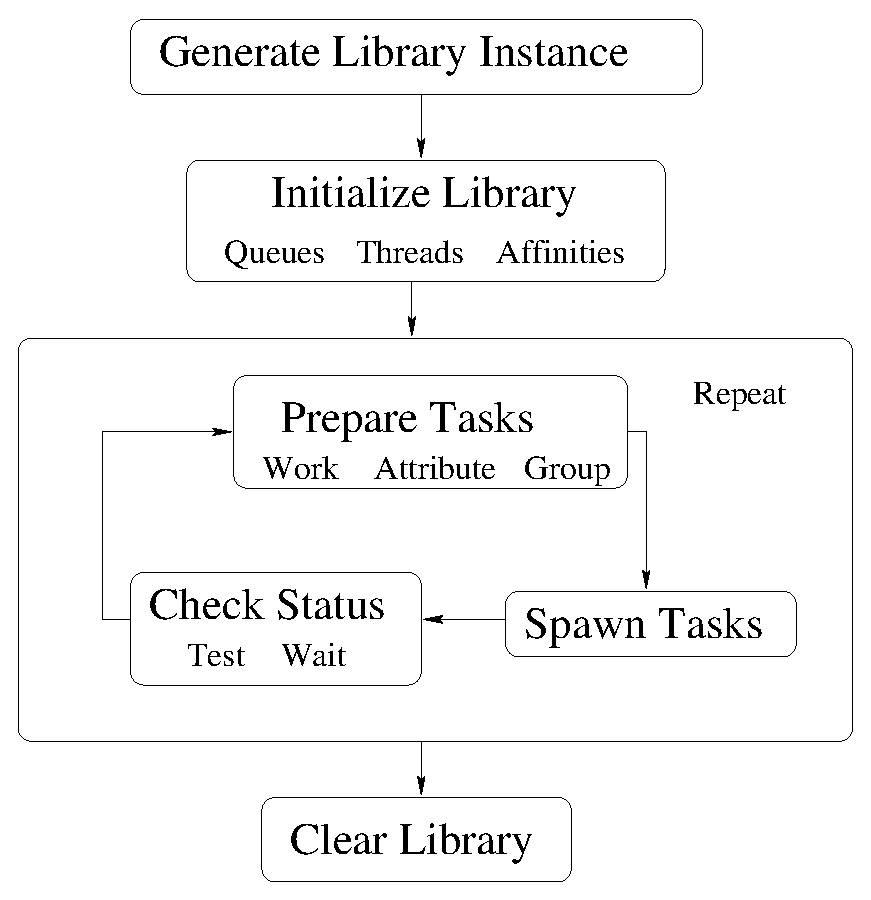
\includegraphics[width=0.5\textwidth]{figs/life-cycle}
\label{fig:life_cycle}
\end{figure}
\end{frame}

\begin{frame}
\frametitle{Generating library instance description}
\begin{itemize}
\item Users can choose library behavior at compile-time.
  \begin{itemize}
  \item Much like the \Cpp{} Standard Library (SL).
  \item Eg., \code{std::vector<int>}.
  \end{itemize}
\item Three (explicit) important \textcolor{blue}{features}.
\end{itemize}
\begin{center}
\tablefont
\begin{tabular}{|c|l|}
\hline
\textcolor{blue}{Feature} & Explanation \\
\hline
\textcolor{blue}{Scheduling policy} & Determines task scheduling. \\
\hline
\textcolor{blue}{Compare} & Determines task ordering. \\
\hline
\textcolor{blue}{Priority} & \textcolor{red}{Nested} within \textcolor{blue}{Compare}. \\
                           & Can be \textit{any} valid type. \\
\hline
\textcolor{blue}{Function Object} & Work that needs to be parallelized \\
\hline
\end{tabular}
\normalsize
\end{center}
\begin{itemize}
\item PFunc provides default values for common cases.
\end{itemize}
\end{frame}

\begin{frame}[fragile]
\frametitle{An example}
\framesubtitle{Cilk-style scheduling}
\begin{center}
\begin{minipage}{0.85\textwidth}
\begin{lstlisting}[basicstyle=\tablefont]
typedef pfunc::generator<cilkS, /* scheduling policy */
                         pfunc::use_default, /* compare */
                         pfunc::use_default> my_pfunc; /*function object*/
\end{lstlisting}
\end{minipage}
\end{center}
\begin{itemize}
\item All types are under the \textcolor{blue}{\code{pfunc}} namespace.
\item Type \textcolor{blue}{\code{generator}} generates library instance description.
\item Default values are specified using \textcolor{blue}{\code{use_default}}.
\end{itemize}
\begin{center}
\tablefont
\begin{tabular}{|c|c|}
\hline
Feature & Default \\
\hline
\textcolor{blue}{Scheduling policy} & \code{cilkS} \\
\hline
\textcolor{blue}{Compare} & \func{std::less<int>} \\
\hline 
\textcolor{blue}{Function object} & \code{struct \{ virtual void operator()() = 0; \};} \\
\hline
\end{tabular}
\normalsize
\end{center}
\end{frame}

\begin{frame}[fragile]
\frametitle{More features}
\begin{itemize}
\item Predefined task scheduling policies.
\end{itemize}
\begin{center}
\tablefont
\begin{tabular}{|c|l|l|}
\hline
\textcolor{blue}{Sched policy} & Explanation & \textcolor{blue}{Compare/Priority} \\
\hline
\textcolor{blue}{cilkS} & Cilk-style scheduling & Not used \\
\hline
\textcolor{blue}{prioS} & Priority-based scheduling & \textcolor{red}{Used} \\
\hline
\textcolor{blue}{proxS} & Proximity-based scheduling using k-d tree & \textcolor{red}{Used} \\
\hline
\textcolor{blue}{fifoS} & Queue-based scheduling & Not used \\
\hline
\textcolor{blue}{lifoS} & Stack-based scheduling & Not used \\
\hline
\end{tabular}
\normalsize
\end{center}
\begin{itemize}
\item Users can also define their very own scheduling policies.
\item \textcolor{blue}{Function object} feature eliminates virtual function
      calls.
\end{itemize}
\end{frame}

\begin{frame}
\frametitle{Important nested types}
\begin{itemize}
\item Library instance description generates \textcolor{red}{four} nested
types.
  \begin{itemize}
  \item Completely encapsulate all requirements for parallelization.
  \end{itemize}
\end{itemize}
\begin{center}
\tablefont
\begin{tabular}{|c|l|}
\hline
\textcolor{blue}{Concept} & Explanation \\
\hline
\textcolor{blue}{taskmgr} & $\ast{}$ Encapsulates PFunc's runtime. \\
          & $\ast{}$ Threads, queues and scheduling policy. \\
\hline 
\textcolor{blue}{attribute} & $\ast{}$ Attached to each task. \\
          & $\ast{}$ Priority, affinity, group affiliation, etc \\
          & $\ast{}$ Default values can be used (eg., Fibonacci). \\
\hline
\textcolor{blue}{group} & $\ast{}$ Used for SPMD-style programming. \\
      & $\ast{}$ Point-to-point, barrier operations. \\
      & $\ast{}$ Default values can be used (eg., Fibonacci). \\
\hline
\textcolor{blue}{task} & $\ast{}$ Handle to a spawned ``\textcolor{red}{task}''. \\
     & $\ast{}$ Used for status inspection. \\
\hline
\end{tabular}
\normalsize
\end{center}
\end{frame}

\begin{frame}[fragile]
\frametitle{An example}
\framesubtitle{Generating Cilk-style interface}
\begin{center}
\begin{minipage}{0.85\textwidth}
\begin{lstlisting}[basicstyle=\tablefont]
typedef pfunc::generator<cilkS, /* scheduling policy */
                         pfunc::use_default, /* compare */
                         pfunc::use_default> my_pfunc; /*function object*/

typedef my_pfunc::attribute attribute;
typedef my_pfunc::group group;
typedef my_pfunc::task task;
typedef my_pfunc::taskmgr taskmgr;
\end{lstlisting}
\end{minipage}
\end{center}
$\rightarrow{}$ \textcolor{blue}{Each nested type is explained in the coming
sections.}
\end{frame}

\begin{frame}
\frametitle{Initializing PFunc}
\begin{itemize}
\item Runtime is encapsulated by \textcolor{blue}{\code{taskmgr}}.
  \begin{itemize}
  \item Initializing PFunc $==$ Constructing object of type \textcolor{blue}{\code{taskmgr}}.
  \end{itemize}
\item To initialize, three important parameters are required.
\end{itemize}
\tablefont
\begin{tabular}{|c|c|l|}
\hline
\textcolor{blue}{Parameter} & Value type & Explanation \\
\hline
\textcolor{blue}{Num queues} & \code{unsigned int} & Number of task queues to be used. \\
           &                     & Queues are numbered from 0 to N-1. \\
\hline
\textcolor{blue}{Threads per queue} & \code{unsigned int[]} & Number of threads to work on each queue. \\
                      &                       & Allows an $m\times{}n$ mapping. \\
                      &                       & $1\times{}n$ mapping represents work-sharing. \\
                      &                       & $n\times{}1$ mapping represents work-stealing. \\
\hline
\textcolor{blue}{Thread affinities} & \code{unsigned int[][]} & Thread-processor affinity. \\
                  &                         & Processors are numbered from 0 to N-1. \\
                  &                         & Default values are accepted. \\
\hline
\end{tabular}
\normalsize
\end{frame}

\begin{frame}[fragile]
\frametitle{Example of initializing PFunc}
\begin{lstlisting}[basicstyle=\tablefont]
int main () {
  unsigned int num_queues = 4;
  const unsigned int num_threads_per_queue[] = {1,1,1,1};
  const unsigned int affinities[4][1] = {{0},{1},{2},{3}};

  /* Create a variable of the type taskmgr */
  my_pfunc::taskmgr cilk_tmanager (num_queues, num_threads_per_queue, affinities);
  ...
  return 0; /* cilk_tmanager is destroyed */
}
\end{lstlisting}
\end{frame}

\begin{frame}
\frametitle{Guidelines for initializing}
\begin{itemize}
\item Each application can have more than one PFunc runtime.
  \begin{itemize}
  \item Eg., if you wanted two different scheduling policies.
  \end{itemize}
\item Typically, do not create more threads than processors.
  \begin{itemize}
  \item \textcolor{red}{Might} degrade performance.
  \item Each instance of PFunc's runtime creates its own threads.
  \end{itemize}
\item Set thread affinities only if you are \textcolor{red}{very sure}.
  \begin{itemize}
  \item May get better performance from cache locality.
  \item But, the thread cannot be scheduled elsewhere.
  \end{itemize}
\item Experiment with different combinations.
  \begin{itemize}
  \item Different scheduling policies.
  \item Different $queue\times{}thread$ combinations.
  \end{itemize}
\end{itemize}
\end{frame}

\begin{frame}[fragile]
\frametitle{Thread behavior}
\begin{itemize}
\item Spawned as soon as PFunc's runtime is initialized.
\item Spin a preset number of times for tasks to execute.
  \begin{itemize}
  \item Own queue first, other queues next (\textcolor{blue}{stealing}).
  \item Stealing policy is implicit in scheduling policy.
  \end{itemize}
\item If no task is found after specified number of attempts. 
  \begin{itemize}
  \item Thread yield to the thread scheduler.
  \item Default value is $2\times{}10^6$ attempts.
  \item \textcolor{blue}{Can be changed by the users.}
  \end{itemize}
\end{itemize}
\begin{center}
\begin{minipage}{0.70\textwidth}
\begin{lstlisting}[basicstyle=\tablefont]
unsigned int num_attempts;
pfunc::taskmgr_max_attempts_get (cilk_tmanager, num_attempts);
if (10000 > num_attempts) {
  pfunc::taskmgr_max_attempts_set (cilk_tmanager, 10000);
}
\end{lstlisting}
\end{minipage}
\end{center}
\end{frame}

\begin{frame}[fragile]
\frametitle{Using global runtimes}
$\rightarrow{}$\textcolor{red}{Initialize globally, and omit
\textcolor{blue}{\code{taskmgr}} from function calls!}
\begin{itemize}
\item When a single object of type \textcolor{blue}{\code{taskmgr}} suffices.
\end{itemize}
\begin{center}
\begin{minipage}{0.70\textwidth}
\begin{lstlisting}
  /* Create a variable of the type taskmgr */
  my_pfunc::taskmgr cilk_tmanager (num_queues, num_threads_per_queue, affinities);

  /* Initialize the global runtime */
  pfunc::init (cilk_tmanager);

  /* Reset the max attempts made if necessary */
  pfunc::taskmgr_max_attempts_get (num_attempts);
  if (10000 > num_attempts) pfunc::taskmgr_max_attempts_set (10000);

  /* Clears ONLY! the global runtime reference */
  pfunc::clear ();

  return 0; 
}
\end{lstlisting}
\end{minipage}
\end{center}
\begin{itemize}
\item We left out \textcolor{blue}{\code{cilk_taskmgr}} from function calls.
  \begin{itemize}
  \item \textcolor{blue}{\func{taskmgr_max_attempts_set}}.
  \item \textcolor{blue}{\func{taskmgr_max_attempts_get}}.
  \end{itemize}
\end{itemize}
\end{frame}

\begin{frame} 
\frametitle{Spawning tasks}
\begin{figure}
\centering
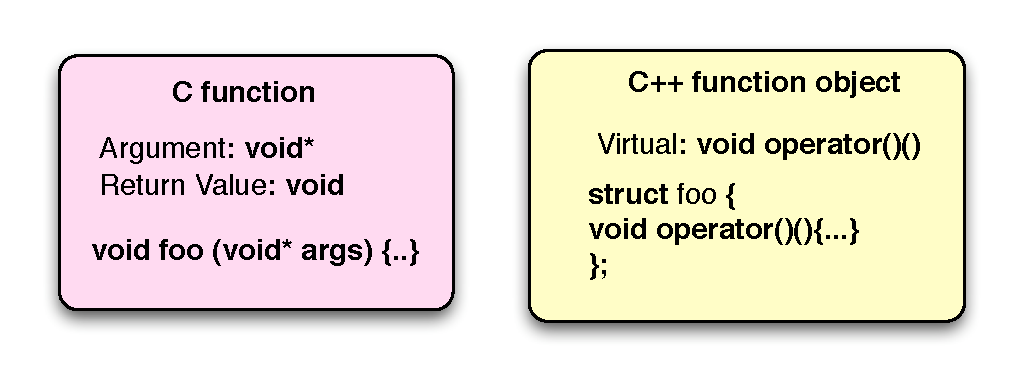
\includegraphics[width=0.7\textwidth]{figs/functors}
\end{figure}
\begin{itemize}
\item For multiple types of function objects, \textbf{OO} helps.
  \begin{itemize}
  \item Virtual function calls cannot be avoided.
  \end{itemize}
\item Spawning a task requires:
  \begin{itemize}
  \item \textcolor{blue}{\code{taskmgr}} $\rightarrow{}$ \textcolor{green}{done}.
  \item \textcolor{blue}{\code{work}} $\rightarrow{}$ \textcolor{green}{done}.
  \item \textcolor{blue}{\code{task}} $\rightarrow{}$ \textcolor{green}{explained here}.
  \item \textcolor{blue}{\code{attribute}} and \textcolor{blue}{\code{group}} $\rightarrow{}$ \textcolor{red}{ignore for now}.
  \end{itemize}
\end{itemize}
\end{frame}

\begin{frame}[fragile]
\frametitle{Fibonacci numbers}
\framesubtitle{Serial version}
\begin{center}
\begin{minipage}{0.5\textwidth}
\begin{lstlisting}
struct fibonacci {
  private:
  const int n;
  int fib_n;

  public:
  fibonacci (const int& n) : n(n), fib_n(0) {}

  int get_number () const { return fib_n; }

  void operator () (void) {
    if (0 == n || 1 == n) fib_n = n;
    else {
      fibonacci fib_n_1 (n-1);
      fibonacci fib_n_2 (n-2);

      fib_n_1();
      fib_n_2();

      fib_n = fib_n_1.get_number () + fib_n_2.get_number ();
    }
  }
};
\end{lstlisting}
\end{minipage}
\end{center}
\begin{center}
\textcolor{red}{$\rightarrow{}$Its naive and impractical, but please bear with
me!}
\end{center}
\end{frame}

\begin{frame}[fragile]
\frametitle{Fibonacci numbers}
\framesubtitle{Parallel version}
\begin{center}
\begin{minipage}{0.5\textwidth}
\begin{lstlisting}
struct fibonacci {
  private:
  const int n;
  int fib_n;

  public:
  fibonacci (const int& n) : n(n), fib_n(0) {}

  int get_number () const { return fib_n; }

  void operator () (void) {
    if (0 == n || 1 == n) fib_n = n;
    else {
      fibonacci fib_n_1 (n-1);
      fibonacci fib_n_2 (n-2);
      task tsk1, tsk2;

      pfunc::spawn (tsk1, fib_n_1);
      pfunc::spawn (tsk2, fib_n_1);

      pfunc::wait (tsk1);
      pfunc::wait (tsk2);

      fib_n = fib_n_1.get_number () + fib_n_2.get_number ();
    }
  }
};
\end{lstlisting}
\end{minipage}
\end{center}
\end{frame}

\begin{frame}[fragile]
\frametitle{Fibonacci numbers}
\framesubtitle{Optimized parallel version}
\begin{center}
\begin{minipage}{0.5\textwidth}
\begin{lstlisting}
struct fibonacci {
  private:
  const int n;
  int fib_n;

  public:
  fibonacci (const int& n) : n(n), fib_n(0) {}

  int get_number () const { return fib_n; }

  void operator () (void) {
    if (0 == n || 1 == n) fib_n = n;
    else {
      fibonacci fib_n_1 (n-1);
      fibonacci fib_n_2 (n-2);
      task tsk1;

      pfunc::spawn (tsk1, fib_n_1);
      fib_n_2();

      pfunc::wait (tsk1);

      fib_n = fib_n_1.get_number () + fib_n_2.get_number ();
    }
  }
};
\end{lstlisting}
\end{minipage}
\end{center}
\begin{center}
\textcolor{red}{$\rightarrow{}$Eliminated half the task creation overhead!}
\end{center}
\end{frame}

\begin{frame}[fragile]
\frametitle{Attributes}
\begin{itemize}
\item Not all tasks are created the same.
  \begin{itemize}
  \item Well, the \textcolor{blue}{Fibonacci} ones are.
  \end{itemize}
\item Control execution of spawned tasks using attributes.
\end{itemize}
\begin{center}
\tablefont
\begin{tabular}{|c|l|}
\hline
\textcolor{blue}{Attribute} & Explanation \\
\hline
\textcolor{blue}{Priority} & Task's scheduling (policy-based). \\
                           & Used only in \code{prioS} and \code{proxS}. \\
\hline
\textcolor{blue}{Queue Number} & Queue on which the task is spawned. \\
                               & Spawned on \textcolor{blue}{current thread's queue} by default. \\
\hline
\textcolor{blue}{Num Waiters} & Number of task completion notifications generated. \\
                              & Enables DAG executions. \\
                              & \textcolor{blue}{$1$} is the default value. \\
\hline
\textcolor{blue}{Nested} & Task is nested (recursively parallel). \\
                          & \textcolor{blue}{\code{True}} by default. \\
\hline
\textcolor{blue}{Grouped} & Task belongs to a group. \\
                          & Grouped tasks can execute SPMD-style. \\
                          & \textcolor{blue}{\code{False}} by default. \\
\hline
\end{tabular}
\normalsize
\end{center}
\end{frame}

\begin{frame}[fragile]
\frametitle{Fibonacci numbers}
\framesubtitle{An example of using attributes.}
\begin{center}
\begin{minipage}{0.5\textwidth}
\begin{lstlisting}
struct fibonacci {
  ...
  void operator () (void) {
    ...
    else {
      fibonacci fib_n_1 (n-1), fibonacci fib_n_2 (n-2);
      task tsk1;
      attribute attr1;
      
      pfunc::attr_nested_set (attr1, true);
      pfunc::attr_grouped_set (attr1, false);

      pfunc::spawn (tsk1, attr1, fib_n_1);
      ...
\end{lstlisting}
\end{minipage}
\end{center}
\begin{itemize}
\item Many ways to set and get attribute values.
  \begin{itemize}
  \item Constructors, independent functions, etc.
  \item Eg., \textcolor{blue}{\func{attr_nested_set}} and
        \textcolor{blue}{\func{attr_grouped_set}}.
  \end{itemize}
\item In the Fibonacci example, these were defaults anyway!
\end{itemize}
\end{frame}

\begin{frame}
\frametitle{Groups}
\begin{itemize}
\item Allows mixing SPMD and task parallel programming.
\item Tasks can communicate through:
  \begin{itemize}
  \item Point-to-point and collective operations.  
    \begin{itemize}
    \item Currently, only \textcolor{blue}{\func{barrier}} is available.
    \end{itemize}
  \end{itemize}
\item Operate at the task-level (not thread-level).
\item Reduce risk of deadlocks from using \textcolor{red}{locks}.
\end{itemize}
\begin{center}
\tablefont
\begin{tabular}{|c|c|l|}
\hline
\textcolor{blue}{Attribute} & Explanation & Type \\
\hline
\textcolor{blue}{Id} & Identification of the group. & \code{unsigned int} \\
          & Useful for debugging purposes. & \\
\hline
\textcolor{blue}{Size} & Maximum number of members. & \code{unsigned int} \\
\hline
\textcolor{blue}{Barrier type} & Type of barrier executed. & \code{enum}: BARRIER\_SPIN (default), \\
                    &                           & BARRIER\_STEAL, BARRIER\_WAIT\\
\hline
\textcolor{blue}{Rank} & Rank of a task in the group. & \code{unsigned int} \\
            & Stored outside the group. & \\
\hline
\end{tabular}
\normalsize
\end{center}
\end{frame}

\begin{frame}[fragile]
\frametitle{Hello world}
\begin{center}
\begin{minipage}{0.55\textwidth}
\begin{lstlisting}
struct parallel_foo {
  void operator()() {
    unsigned int rank, size;
    pfunc::group_rank(rank);
    pfunc::group_size(size);
    std::cout << "Hello world: " << rank << " of " << size << std::endl;
  }
};

int main () {
  parallel_foo work[10];
  my_pfunc::group group;
  my_pfunc::attr attr;
  ...
  pfunc::attr_grouped_set (attr, true);
  pfunc::group_size_set (group, 10);
  for (int i=0; i<10; ++i) {
    work[i].initialize (i);
    pfunc::spawn (tasks[i], attr, group, work[i]);
  }
  ...
}
\end{lstlisting}
\end{minipage}
\end{center}
\begin{itemize}
\item Each \textcolor{blue}{\code{parallel_foo}} is launched with a group.
\item \textcolor{blue}{\func{group_rank}} and \textcolor{blue}{\func{group_size}} infer group from context.
  \begin{itemize}
  \item Assuming a global runtime has been set.
  \end{itemize}
\end{itemize}
\end{frame}

\begin{frame}[fragile]
\frametitle{Exceptions}
\begin{itemize}
\item Implement a robust exception handling mechanism.
\item Extend \textcolor{blue}{\code{std::exception}}.
\item \textcolor{blue}{Exceptions are delivered to the calling site.}
  \begin{itemize}
  \item \textcolor{red}{Caller/callee may not be in the same thread!}
  \item Deliver to each waiting task.
  \end{itemize}
\end{itemize}
\begin{center}
\begin{minipage}{0.60\textwidth}
\begin{lstlisting}
struct my_fn_object { 
  void operator () { 
    try { 
      ... 
    }
    catch (const pfunc::exception& error) { 
      std::cout << "Description: " << error.what () << std::endl;
      std::cout << "Trace: " << error.trace () << std::endl; 
      std::cout << "Code: " << error.code () << std::endl;
    } 
  }
};
\end{lstlisting}
\end{minipage}
\end{center}
\end{frame}

\begin{frame}[fragile]
\frametitle{Integrating with PFunc's exceptions}
\begin{center}
\begin{minipage}{0.60\textwidth}
\begin{lstlisting}
struct my_fn_object { 
  void operator () { 
    try { 
      ... 
    }
    catch (const pfunc::exception& error) { 
      pfunc::exception* clone = error.clone();
      clone->append (": from my_fn_object at " PFUNC_FILE_AND_LINE()); 
      clone->rethrow ();
    } 
  }
};
\end{lstlisting}
\end{minipage}
\end{center}
\begin{itemize}
\item Preserve across threads.
  \begin{itemize}
  \item \Cpp{}0x handles this within the language.
  \end{itemize}
\item Exception handling is \textcolor{red}{disabled} by default.
  \begin{itemize}
  \item Performance, performance, performance. 
  \end{itemize}
\end{itemize}
\end{frame}

\begin{frame}
\frametitle{Performance monitoring}
\begin{center}
\textcolor{red}{Critical step in developing industrial strength code!}
\end{center}
\begin{itemize}
\item Fully integrated with PAPI.
  \begin{itemize}
  \item Open-source, proven, portable.
  \end{itemize}
\item Allows users to measure specific application statistics.
\item Events are initialized during runtime initialization.
  \begin{itemize}
  \item Derive from \textcolor{blue}{\code{perf_data}}.
  \item Pass it during construction of \textcolor{blue}{\code{taskmgr}}.
  \end{itemize}
\end{itemize}
\end{frame}

\begin{frame}
\frametitle{Conclusions}
\begin{itemize}
\item PFunc increases support for:
  \begin{itemize}
  \item Modern HPC applications.
  \item Modern computer architectures.
  \item SPMD-style programming.
  \item \textcolor{blue}{DAG execution, frequent pattern mining, sparse CG.}
  \end{itemize}
\item Future work.
  \begin{itemize}
  \item \textcolor{red}{Parallelize more applications!}
  \item Increase support for GPGPUs.
  \end{itemize}
\end{itemize}
\vspace{+10pt}
\begin{center}
\textcolor{red}{$\ast{}$ If you have an application, we will help you 
                parallelize. $\ast{}$}
\end{center}
\end{frame}

\begin{frame}
\frametitle{The End}
\begin{center}
\textcolor{blue}{Thanks for your attention!}
\end{center}

\tiny
{Publications:} \\
\begin{picture}(2,2)
\put(0,0){\line(1,0){470}}
\end{picture}
\begin{itemize}
\item 
P. Kambadur, A. Gupta, A. Ghoting, H. Avron and A. Lumsdaine.
{\bf{\em ``PFunc: Modern Task Parallelism For Modern High Performance Computing.''}}
{\em SC, 2009.}
\item 
P. Kambadur, A. Ghoting, A. Gupta and A. Lumsdaine.
{\bf{\em ``Extending Task Parallelism For Frequent Pattern Mining.''}}
{\em ParCo, 2009.}
\item 
P. Kambadur, A. Gupta, T. Hoefler and A. Lumsdaine.
{\bf{\em ``Demand-driven Execution of Static Directed Acyclic Graphs 
Using Task Parallelism.''}}
{\em Submitted to the HiPC, 2009.}
\end{itemize}
\normalsize
\end{frame}

\begin{frame}[fragile]
\frametitle{Fibonacci: task creation overhead.}
$\rightarrow{}$ \textcolor{blue}{Fibonacci number 37 ($2^{36}\approx{}69$ billion tasks).}
\tablefont
\begin{center}
\begin{tabular}{|c|c|c|c|c|} 
\hline
Threads & Cilk Time (secs) & PFunc/Cilk & TBB/Cilk & PFunc/TBB \\
\hline
1  & 2.17 & 2.2178  & 4.431 & 0.5004 \\ 
\hline
2  & 1.15 & 2.1135 & 4.1924 & 0.5041 \\ 
\hline
4  & 0.55 & 2.2131 & 4.4183 & 0.5009 \\ 
\hline
8  & 0.28 & 2.2114 & 4.9839 & 0.4437 \\ 
\hline
16 & 0.15 & 2.4944 & 5.9370 & 0.4201 \\ 
\hline
\end{tabular}
\end{center}
\normalsize
\begin{itemize}
\item \textcolor{red}{2x faster than TBB!}
\item Only 2x slower than Cilk.
  \begin{itemize}
  \item \textcolor{red}{But provides more flexibility!}
    \begin{itemize}
    \item Fibonacci is the \textcolor{red}{worst} case behavior.
    \end{itemize}
  \item Library-based rather than a custom compiler.
  \end{itemize}
\end{itemize}
\tiny\textcolor{blue}{$\ast{}$4 socket, quad-core AMD 8356 with Linux 2.6.24.}\normalsize
\end{frame}

\begin{frame}[fragile]
\frametitle{Results}
\framesubtitle{Custom task scheduling and priority: frequent pattern mining.}
\begin{figure}
\includegraphics[width=0.8\textwidth]{figs/fim_8}
\label{fig:fim}
\end{figure}
\end{frame}

\begin{frame}[fragile]
\frametitle{Results}
\framesubtitle{Task groups: iterative sparse solvers.}
\begin{figure}
\includegraphics[width=0.9\textwidth]{figs/cg_8}
\label{fig:cg}
\end{figure}
\end{frame}

\begin{frame}[fragile]
\frametitle{Results}
\framesubtitle{Multiple completion notifications: DAG execution (runtime).}
\begin{figure}
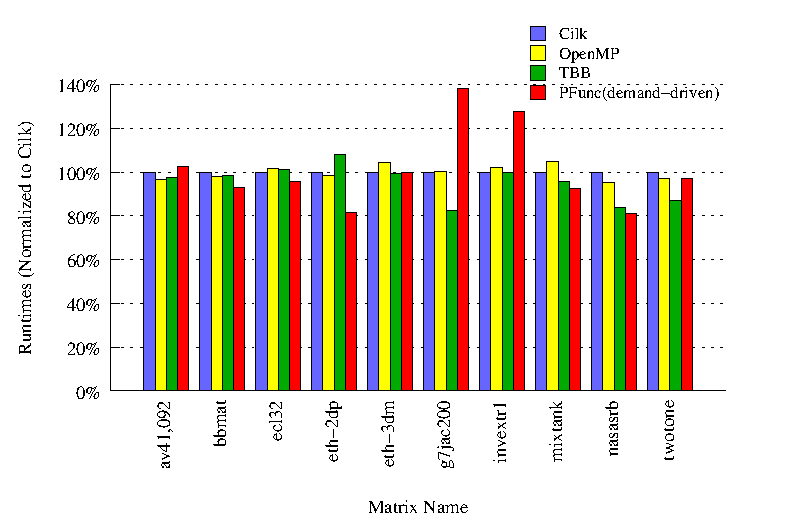
\includegraphics[width=0.9\textwidth]{figs/dag_speedup}
\label{fig:dag_speedup}
\end{figure}
\end{frame}

\begin{frame}[fragile]
\frametitle{Results}
\framesubtitle{Multiple completion notifications: DAG execution (peak memory).}
\begin{figure}
\includegraphics[width=0.9\textwidth]{figs/dag_memory}
\label{fig:dag_memory}
\end{figure}
\end{frame}

\end{document}
